\chapter{Project Schedule}
In this section the project schedule is shown. It has been implemented from a Gantt chart, attached on the next page.

This project is focused in developing a complete space sensor platform with an on ground post-processing interface. For that reason on the project schedule tu critical path are observed. 

First one, corresponds to project management, administrative and communication tasks. These tasks are all project duration tasks, because if one of these tasks stops all project is affected. These tasks are essential to coordinate and to carry out the project.

Second critical path, is related with the development of the sensor platform and is not as easy to see as the first one. The whole project is been structured with fix date milestones in order to control deadlines and progress.

\begin{landscape}
	\begin{figure}[H]
	\centering
	\begin{tabular}{@{}c@{\hspace{.5cm}}c@{}}
		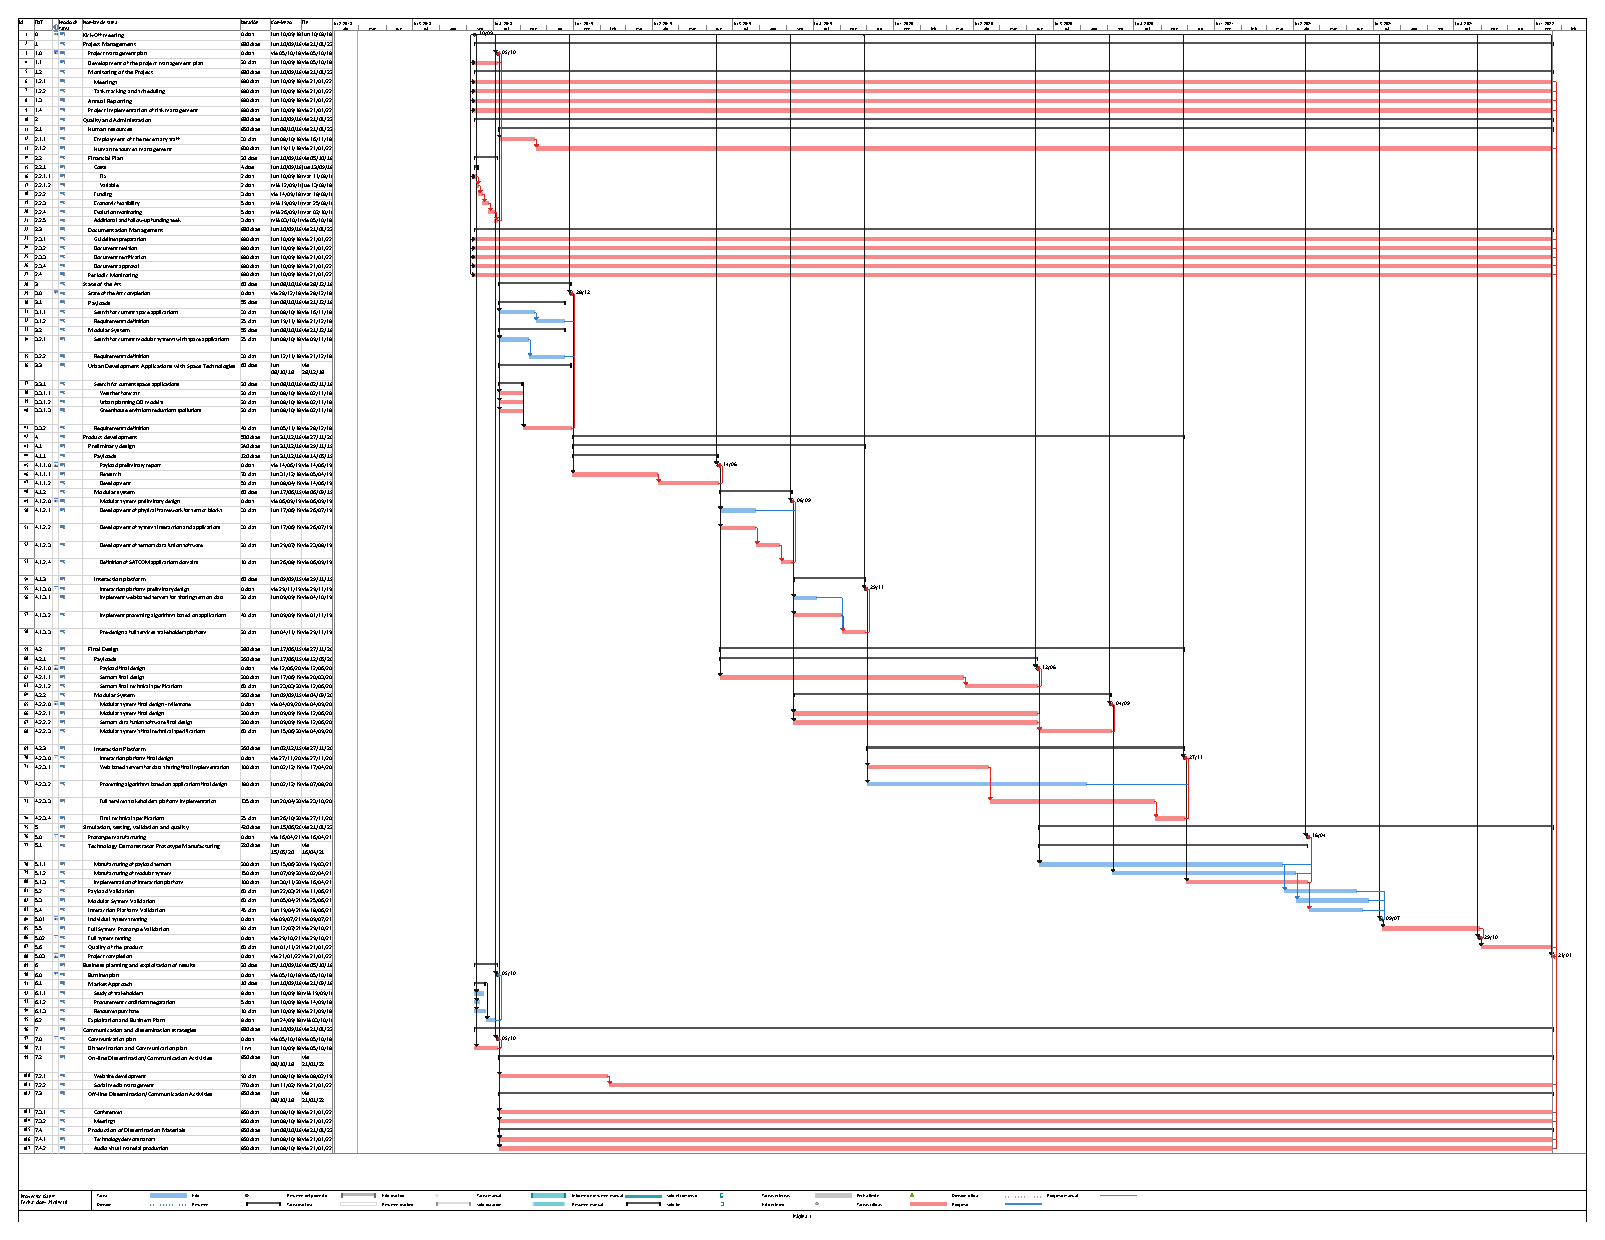
\includegraphics[page=1,width=1.2\textwidth]{./images/gantt/GANTT.pdf}
	\end{tabular}
	\caption{Gantt chart}
	\label{Gantt}
	\end{figure}
\end{landscape}